\chapter{Vortices in superconductors}
\label{sec:Vor}
% Brain-log:
% Topological defects
% Cause of phase-transitions; vortex blow-out
% Abikosov vortices
%
\noindent In conventional type-I superconductors, the Meissner effect prevents any magnetic field from penetrating the superconductor when it is in the
superconducting state. In a type-II superconductor, the transition between the normal- and superconducting state is more gradual than in the type-I case
due to an intermediate transitional state where topological defects in the superconducting field  becomes stable allowing quanta of magnetic field
to pass through the material. The transitional value of the external field strength below which no magnetic field penetrates the superconductor is
called $B_{c1}$. The upper transitional field strength above which the material stops being superconducting altogether is called $B_{c2}$. The state
with regions of topological defects through which magnetic field quanta can penetrate, which are interspersed in a sea of
superconducting state then exists between these values. It is important to note that the Meissner effect is still present in this transitional state - preventing magnetic field
lines from penetrating the superconducting state, however at topological defects, the material switches to the normal state and thus
allows magnetic field lines to penetrate at these points. The final continuous transition to the normal state at $B_{c2}$ is then caused by the
proliferation of vortex-loops, sending the whole material to the normal state.
%TODO: cite.

The regions of normal state containing a topological defect of the superconducting state and through which magnetic field quanta can penetrate are known
as superconducting vortices because they are surrounded by a circulating superconducting current. This current is set up by the presence of the magnetic field
and shields the rest of the superconducting condensate from its influence.

Whether a superconductor is considered type-I or type-II is conventionally given by the magnetic field penetration length $\lambda$ and the superconducting
coherence length $\xi$ which come together to form the \ac{gl} parameter $\kappa = \lambda/\xi$.
These parameters come out of the description of the superconducting state given by the \ac{gl} theory of a single-component complex field minimally coupled
to a gauge field.
If $\kappa\gg1$ then we say we have a strongly
type-II superconductor, while is $\kappa\ll1$ the superconductor is strongly type-I. The transitional value between type-I and type-II have a theoretical
mean-field value of $\kappa = 1/\sqrt{2}$, however numerical calculations has given it the value $\kappa = (0.76\pm0.04)/\sqrt{2}$ all within the conventional
\ac{gl} formalism.

In a type-II conventional superconductor without any structural defects, as we increase the field strength, we introduce more vortices into the material
in order to carry the required number of magnetic field quanta. At first these vortices behave like a liquid where they mutually repel each other if they 
get close. As more vortices are introduced to the system, the inter-portex repulsion leads to them forming a two-dimensional lattice with equidistant lattice-spacing.
Since the triangular lattice is the lattice with the highest packing fraction, i.e. the lattice that have the highest density of sites at a given lattice spacing,
the lattice formed will be triangular. Such a triangular (hexagonal) lattice of single quanta vortices is known as the Abrikosov lattice since it consists
of single quanta vortices which are known as Abrikosov vortices.

\section{Vorticity observables}
\label{sec:Vor:Obs}

% Local vorticity
% Total vorticity when going around the system and why
%    we have restrictions on the filling fraction.

A condensate described by a complex field $\psi$ with phase $\theta$ can have topological defects given by discontinuities in the field $\theta$ due to its compact
nature ($\theta\in[0,2\pi)$). Such topological defects can be quantified by a non-zero winding-number $N_v$ which measures how the phase $\theta(\v{r})$ moves around the
unit circle as we change the position $\v{r}$ in a closed loop around the defect. These topologicals
defects then lead to singularities in the field $\nabla\theta$ which allows a nonzero value of $\nabla\times\nabla\theta$ at these points\footnote{From vector calculus
we know that for a continuously differentiable field $f(\v{r})$, it is the case that $\nabla\times\nabla f = 0\;\forall\v{r}$.}%
. Integrating over a surface
$S$ with surface normal vector $\hat{s}$ of the system and using Stokes theorem then yields
\begin{equation}
    \label{eq:Vor:Obs:vorticityIntegral}
    \int_S\!\mathrm{d}^2r (\nabla\times\nabla\theta)\cdot\hat{s} = \oint_{\partial S}\nabla\theta\cdot\mathrm{d}\v{r} = 2\pi N_v,\quad N_v\in\mathbb{Z},
\end{equation}
where $\partial S$ is a path around the boundary of $S$ traversed counter-clockwise. The last equality comes from the observation that
$\partial S$ is far away from the singularity such that $\nabla\theta$ is continuous along the path and $N_v$ thus counts the number of times the vector $\theta$
rotates counter-clockwise back to its initial position. If there is no topological defect inside the boundary $\partial S$ then $\theta$ will increase as much as it
decreases along the path, such that $N_v=0$. If a topological defect in the form of a vortex is present, then $N_v\neq0$ \cite{Smorgrav052}.
$N_v$ can then be interpreted as the total vorticity of the field $\theta$ over the surface $S$.
Since $N_v$ is the total vorticity which can consist of several individual defects, then from Eq.~\eqref{eq:Vor:Obs:vorticityIntegral} we see that
\begin{equation}
    \label{eq:Vor:Obs:localVorticity}
    \v{n}_v = \frac{\nabla\times\nabla\theta}{2\pi} 
\end{equation}
must be interpreted as a vector of local vorticity density.

If the system described above contains a gauge field that is coupled to $\psi$, then any meaningful observable needs to be gauge-invariant.
We clearly see that the expression in Eq.~\eqref{eq:Vor:Obs:localVorticity} is gauge-dependent by sending $\theta\to\theta+\phi$. To make a gauge-invariant observable under
the gauge-transformation in Eq.~\eqref{eq:LM:Derivatives:gaugeTransformation}, we see that we need to modify the definition to
\begin{equation}
    \label{eq:Vor:Obs:localGaugeVorticity}
    \v{n}_v = \frac{\nabla\times(\nabla\theta + g\v{A})}{2\pi}.
\end{equation}
This expression then defines $\v{n}_v$ as a gauge invariant vector of local vorticity density of the compact field $\theta$.

In lattice models we want to discretize the vorticity density in Eq.~\eqref{eq:Vor:Obs:localGaugeVorticity} in order to effectively calculate it in \ac{mc} simulations
of the lattice model. In such a discrete model we have to take care to re-compactify the quantity $\nabla\theta+g\v{A}$ to only be defined on some interval of length $2\pi$.
Using the discretization mapping of $\partial_\mu$ and $A_\mu(\v{r})$ from Eq.~\eqref{eq:LM:Field:Fluc:discretization}, we want
$\Delta_\mu\theta + gA_{\v{r},\mu}\in[-\pi,\pi)$. Defining the operator
\begin{equation}
    \label{eq:Vor:Obs:moduloOperator}
    \hat{C}_\pi\, x = \modulo(x+\pi,2\pi)-\pi,
\end{equation}
the discretized vorticity density can be written
\begin{equation}
    \label{eq:Vor:Obs:discreteLocalVorticity}
    \begin{split}
        \v{n}_{v,\v{r}} &= \frac{\hat{e}_\mu\epsilon_{\mu\nu\lambda}\Delta_\nu\hat{C}_\pi(\Delta_\lambda\theta_\v{r} + gA_{\v{r},\lambda})}{2\pi a^2}\\
        &= \frac{1}{2\pi a^2}\sum_\mu \hat{e}_\mu\sum_{\boxdot_\mu}\hat{C}_\pi(\Delta_\lambda\theta_\v{r} + gA_{\v{r},\lambda}).
    \end{split}
\end{equation}
Implicit summation over repeated indices is used on the first line while on the second, the components of the vector $\v{n}_{v,\v{r}}$ are written as plaquette-sums,
which are sums of direction dependent quantities along a path $\boxdot_\mu$, which is described below Eq.~\eqref{eq:LM:Field:Fluc:plaquetteSum} and illustrated in
Figure~\ref{fig:LM:Field:Fluc:plaquetteSum}. In the plaquette-sum the directional quantity is always chosen along the path and the path is traversed according to
the right hand rule with normal vector $\hat{e}_\mu$ \cite{Kragset08,shimizu12}.

If the lattice system has an external field that yields a filling fraction $f$, \eg produced by one of the gauges in Section~\ref{sec:LM:Field}, then each plaquette-sum
in Eq.~\eqref{eq:Vor:Obs:discreteLocalVorticity} will have a contribution $f/a^2$. To see this assume \eg that $\theta_\v{r}$ is the same everywhere such that
$\Delta_\lambda\theta_\v{r}=0$ and insert the Landau gauge from Eq.~\eqref{eq:LM:Field:LandauGauge} into the $z$-component of $\v{n}_{v,\v{r}}$. This yields $f/a^2$.
Hence, to assure that the vortex observable yields the actual vortex quanta integer values when evaluated on a lattice with a uniform external field in the $z$
direction with filling fraction $f$, we have to use the lattice function
\begin{equation}
    \label{eq:Vor:Obs:discreteLocalVorticity:fieldSubtracted}
    n^z_\v{r} = (\v{n}_{v,\v{r}})_z - \frac{f}{a^2}.
\end{equation}

If the system consists of multiple condensate components $\psi^h = \rho^he^{i\theta^h}$, then we can define a separate vorticity flux density $n^{z,h}_\v{r}$ for each component
$h$ by letting $\theta\mapsto\theta^h$ in the definitions of $n^z_\v{r}$ in Eqs.~\eqref{eq:Vor:Obs:discreteLocalVorticity} - \eqref{eq:Vor:Obs:discreteLocalVorticity:fieldSubtracted}.


\section{Unconventional vortices}
\label{sec:Vor:UnconventionalVortices}

In a conventional superconductor, the isotropic (\ie $s$-wave) nature of the superconducting state implies that stable vortices can only contain a single quanta of magnetic flux.
In other words, if through some random thermal fluctuation a defect appears that contains $n$ quanta of magnetic flux, this will soon decay into $n$ individual vortices,
which each contain a single quanta and which we thus call single-quanta vortices.
For the individual stable topological defects to contain
multiple quanta of magnetic flux, the superconducting state has to be unconventional in some way.
One way in which a superconductor can host stable multiple quanta vortices is if the superconducting state for some reason has an unconventional symmetry. This could \eg be
caused by unconventional (\ie non-phononic) mechanisms of Cooper-pair formation such as van der Waahls- or spin-mediated interaction \cite{Sigrist05}.
In this case multiple components might be needed in order to describe the symmetry which can result in the stabilization of vortices with double as well as fractionalized
quanta \cite{Babaev02}.

A more specific example is that this can happen when a magnetic field penetrates a sample of material that is in a $p+ip$ superconducting state, \ie a state where the
pairing function is described by two components that each have a $k_x\pm ik_y$ dependence on the crystal momentum $\v{k}$ in the continuum limit. The linear
$k$-dependence implies a finite angular momentum of the Cooper pairs with $l=1$ and the phases of the components are locked by an angular momentum difference $\Delta l=2$.
This has the consequence $n_+ = n_- + 2$ on any non-trivial winding numbers $n_+$ and $n_-$ of the two different components which implies that if a vortex exists some
place where the sub-dominant component has winding number $n_-=0$, then the dominant component must have $n_+=2$ and thus the vortex must be a double quantum vortex%
\footnote{It is the winding number of the dominant component that determines the number of magnetic flux quanta that the vortex is allowed to contain because the sub-dominant
component is zero in locations far away from the vortex core by the nature of being sub-dominant. Thus, it doesn't contribute to the closed loop integral in 
Eq.~\eqref{eq:Vor:Obs:vorticityIntegral} when integrating the supercurrent in a circle around the vortex.}.

In the type of superconductor described above, the winding numbers $n_+$ and $n_-$ fully determine the structure of possible vortices. In the following we will use the
notation $(n_+,n_-)$ to specify these types of vortices. The possibilities for single-quanta vortices in this notation are thus the vortices $(1, -1)$ and $(-1,-3)$.
The latter type has a higher winding number in the sub-dominant component which implies a more complex core structure and has a higher energy cost pr. vortex \cite{Garaud15}
which means that of the two, it is the $(1, -1)$ variety that will be expected to be stable in experiments.

It is also possible to have double quanta vortices, which are either of the $(2, 0)$ or $(-2, -4)$ variety. Again, the type of vortex with the higher winding number in
the sub-dominant component exhibits a more complex core structure. For the choices of various internal parameters of such systems that we have studied, it is the $(2, 0)$
type of vortex that is associated with the lowest energy cost and thus the one that is stable \cite{AsleGaraud16,Garaud15,Sauls09}.

As we have mentioned, the different types of vortices will in general have different types of core-structures even though they may permit the same number of magnetic flux
quanta to penetrate. One diagnostic tool to separate different kinds of vortices is thus to observe the structure of the vortex core. Aside from plotting the actual vorticity
$n_\pm$ of the component through Eq.~\eqref{eq:Vor:Obs:discreteLocalVorticity:fieldSubtracted}, this can done by \eg plotting
the amplitudes of the dominant and sub-dominant component, the phase-difference $\theta_+-\theta_-$ of the different components or the magnetic field in the region of
the vortex core. A rendition of the essential features of plots of dominant component vorticity density $n_+$ and phase-difference is shown in Figure~\ref{fig:Vor:schematic} for the
two vortex types $(1,-1)$ and $(2,0)$. We see from the figure that the double quanta vortex type $(2,0)$ can be distinguished from the single quanta vortex by having an
extended ring of vorticity density, as well as having a core region in the phase difference plot that is rotated by $\pi/2$ radians from the asymptotic value of this phase difference.
These features were used in our work to identify double and single quanta vortices in \ac{mc} simulations.

\begin{figure}[h]
    \newcommand{\fractionwidth}{.38}
    \centering
    \begin{subfigure}[b]{\fractionwidth\textwidth}
        \centering
        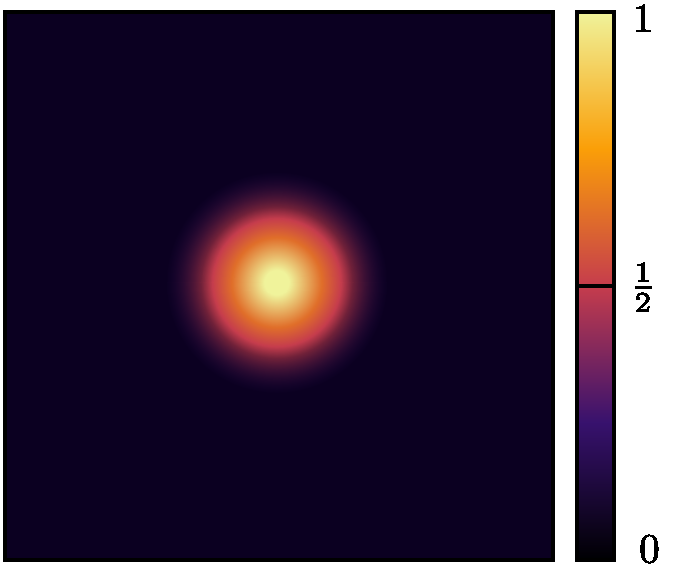
\includegraphics[width=\textwidth]{1q_vorticity.pdf}
        \caption{\label{fig:Vor:schematic:1q:v}}
    \end{subfigure}
    \hspace{2em}
    \begin{subfigure}[b]{\fractionwidth\textwidth}
        \centering
        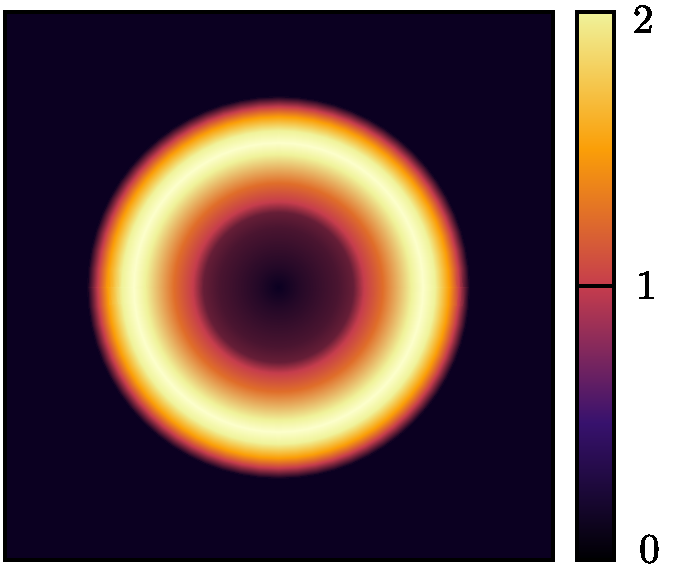
\includegraphics[width=\textwidth]{2q_vorticity.pdf}
        \caption{\label{fig:Vor:schematic:2q:v}}
    \end{subfigure}

    \begin{subfigure}[b]{\fractionwidth\textwidth}
        \centering
        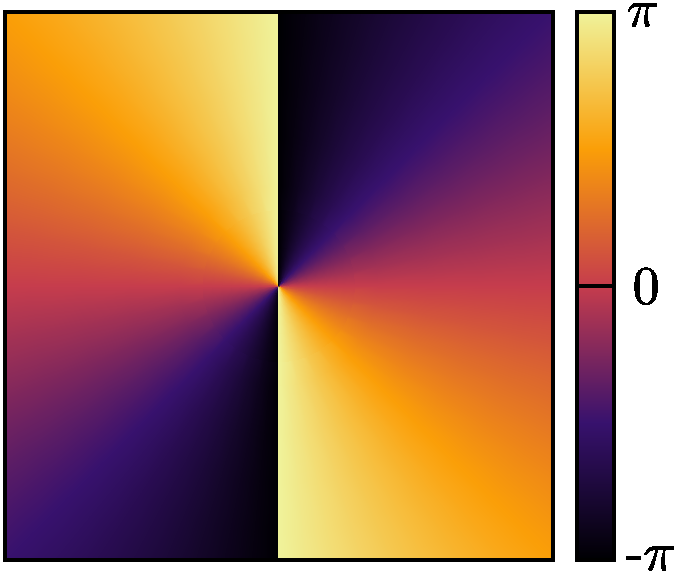
\includegraphics[width=\textwidth]{1q_vortex.pdf}
        \caption{\label{fig:Vor:schematic:1q:pd}}
    \end{subfigure}
    \hspace{2em}
    \begin{subfigure}[b]{\fractionwidth\textwidth}
        \centering
        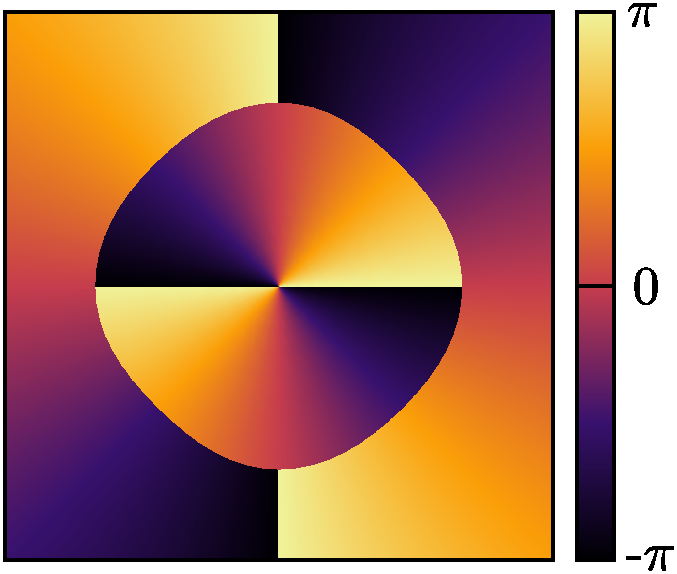
\includegraphics[width=\textwidth]{2q_vortex.pdf}
        \caption{\label{fig:Vor:schematic:2q:pd}}
    \end{subfigure}
    \caption{Schematic of vorticities and corresponding phase difference signature $\theta_+-\theta_-$ of vortices in a system with external magnetic field $\v{B} = B\hat{z}$. 
     \protect\subref{fig:Vor:schematic:1q:v} and \protect\subref{fig:Vor:schematic:1q:pd} shows vorticity and phase-difference respectively for a 
     singly-quantized vortex with winding number $n_+=1$ and $n_-=-1$.
     \protect\subref{fig:Vor:schematic:2q:v} and \protect\subref{fig:Vor:schematic:2q:pd} shows vorticity and phase difference respectively for a doubly-quantized vortex with winding number $n_+=2$ and $n_-=0$. The figures are directly based on the ones presented in Ref.~\cite{AsleGaraud16}.}
    \label{fig:Vor:schematic}
\end{figure}


% A peculiar property of this state is that
% it features spontaneously broken time-reversal symmetry. In terms of the superconducting components, this means that the state can be written in terms of a dominant
% component $\eta_+$ which has a large amplitude throughout when an external field is applied to the material, and a sub-dominant component $\eta_-$ which has zero
% amplitude except at topological defects such as vortices
% or boundaries between normal and superconducting regions of material. These components are tied together through a time-reversal transformation, meaning that one is the
% time-reversed version of the other. Since a magnetic field breaks time-reversal symmetry, the consequence of flipping the direction of the external magnetic field is thus
% that $\eta_-$ becomes the dominant component, while $\eta_+$ becomes sub-dominant. In the absence of an external field, neither component is energetically favored, which
% results in a $\mathbb{Z}_2$ symmetry which becomes spontaneously broken in the superconducting state.


\section{Ensambles of vortices}

With increasing field strength, more quanta of magnetic flux will penetrate the mixed phase and thus it will contain an increasing number of vortices that form flux-lines through the system
. If any structural defects are present in the
system, then this leads to local suppression of the superconducting condensate such that vortices are less energetically costly, and vortices will thus be predominantly located in such regions.
This is called pinning of vortices because these regions attract vortices and since their location is determined by external factors and not by the inter-vortex interactions themselves.
Free vortices are mobile in 
response to an electric current and this leads to energy-loss and resistance in the mixed phase. Pinning regions have the effect of resisting such movement and thus can contribute to increasing
the amount of resistance free current \cite{Ishida19}.

In the absence of such pinning, vortex tubes that run through the material in the direction of an external magnetic field can be ordered in a lattice according to their mutual interaction.
Such a lattice is called an Abrikosov lattice or a flux line lattice since the vortex lines/tubes carry quanta of flux of the external magnetic field.
The Abrikosov lattice then exists in the mixed phase of type-II superconductors and is destroyed when either the temperature or magnetic field strength is increased beyond a certain level
$B_{c2}(T)$ where the material enters the normal non-superconducting phase. This transition can be characterized in terms of a proliferations of unbound vortex loops which destroys the
phase-coherence of the superconducting state \cite{Fossheim-Sudbo-Book}.

If the interaction between the flux lines is weak compared to entropic forces such as thermal fluctuations, then fluctuations of the vortex flux lines can cause melting of the vortex lattice.
In this molten state, the vortex flux lines still interact repulsively which yields an average preferred inter-vortex distance given by the balance between inter-vortex repulsion and the inclusion of the
necessary number of vortices in order to carry the external magnetic field, however any directionally dependent long range correlation is lost. This corresponds to the behavior
of particles in a liquid, and the molten state is thus called a vortex liquid. Such states are commonly found in high-$T_c$ superconductors such as \ce{YBa_2Cu_3O_{7-\delta}}.
The transition between an ordered lattice of vortices and a vortex liquid is known as a vortex lattice melting transition.
This transition can also be achieved by tuning the strength of the magnetic field. This implies a magnetic field strength $B_{c1}$, below which the Meissner effect
completely excludes all magnetic fields, and a strength $B_{M}>B_{c1}$ above which the vortices behave as a liquid, \ie without any long range correlations except that of an average distance.
Finally superconductivity is destroyed at $B_{c2}>B_M$ when a proliferation of vortex loops destroy all vortex correlations and the material enters the normal state.
These different states of the vortex lattice map out a region in the $B-T$ parameter space such as the one shown in Figure~\ref{fig:Vor:phases}.
There also exists intermediate glassy phases of vortex matter between the extremes of a completely ordered lattice and a liquid when pinning of vortices is combined
with low temperature in an external magnetic field \cite{Sanchez19,Koch89}.

\begin{figure}[t]
    \centering
    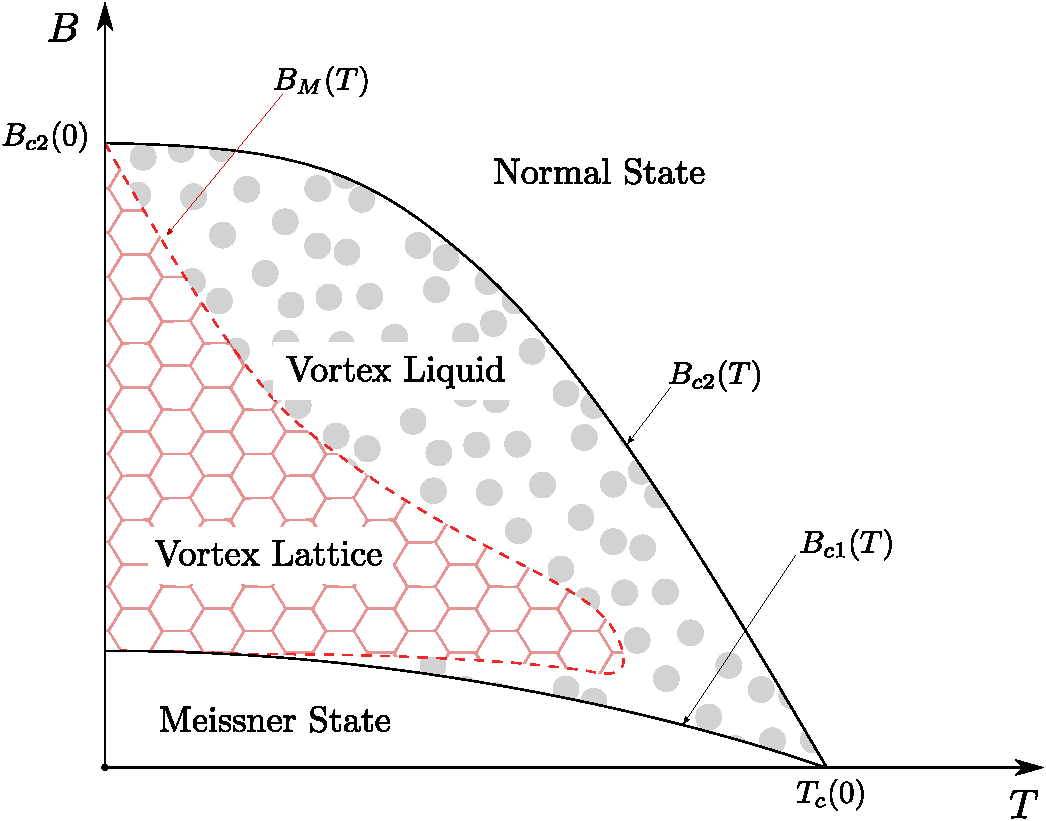
\includegraphics[width=.7\textwidth]{vortex_phases.pdf}
    \caption{Simplified phase diagram of the states of vortex matter in a type-II superconductor in the $B-T$ phase space. This is based on the Lindemann criterion \cite{Sonier98}.}
    \label{fig:Vor:phases}
\end{figure}

The structure and behavior of a flux-line lattice in the mixed phase of a type-II superconductor is dependent on the symmetry and nature of the superconducting phase. In conventional single-component
superconductors with $s$-wave symmetry, the vortices interact asymptotically\footnote{In this context ``asymptotically'' means in the asymptotic limit of large separation between vortices.}
through isotropic repulsion that can be modeled by a modified Bessel function of the second kid \cite{Abrikosov56,Kramer71,Chaves11}. In a clean material, this interaction leads experimentally
to a triangular (hexagonal) lattice of vortices due to this lattice symmetry having the largest packing-fraction of any
two-dimensional lattice, i.e. it is the lattice that gives the highest density of vortices given a set inter-vortex distance and thus give the lowest energy configuration \cite{Cribier66,Essmann67}.
Theory predicts that also a square lattice of single quanta vortices should be possible at higher fields for $\kappa \gtrsim 1/\sqrt{2}$ \cite{Kramer71}, however in the London-approximation,
which is valid at $\kappa\gg1$, the triangular symmetry is the most stable for all fields \cite{Matricon64}.
Interestingly, the vortex lattice symmetry can be incommensurate to the underlying crystal lattice structure.

In theoretical models of unconventional superconductors, such as superconductors with multiple components and non-isotropic symmetry, even more complex behavior of the mixed phase is predicted.
We have already mentioned the appearance of a vortex-liquid state separate from the vortex lattice state in high-$T_c$ superconductors, which are overwhelmingly of the extreme type-II category
and described by a single component unconventional $d$-wave symmetry.
In superconductors with multiple components where each component can be modeled by a conventional London-approximation, a phase transition from the superconducting state to a superfluid state is possible
in the mixed phase by melting of a composite Abrikosov vortex lattice into a state with a remaining ordered neutral mode \cite{Smiseth05}.

\subsection{Vortex matter in $p_x+ip_y$-superconductors}

In our work we have been specifically interested in the vortex matter of superconductors with $p$-wave symmetry. These types of superconductors are described by two components that are intrinsically
coupled and give rise to unconventional composite vortices as described in Section~\ref{sec:Vor:UnconventionalVortices}. The stable single-quanta composite vortices, which are denoted
as vortex type $(1, -1)$ in the notation of Section~\ref{sec:Vor:UnconventionalVortices}, are theoretically predicted to form lattices with square symmetry \cite{Agterberg00,Heeb99,AgterbergVortex98}.
Such symmetry has been observed in the vortex lattice of the unconventional superconductor \ce{Sr2RuO4} \cite{Riseman98,Aegerter98,Ray14,Curran11} and is thus part of the body of evidence
supporting a $p$-wave symmetry of the superconducting state of this material. The theoretical predictions are supported by numerical calculations that also show that at lower fields
a triangular vortex lattice consisting of double-quanta $(2,0)$-vortexes is the preferred configuration \cite{AsleGaraud16}. Since these calculations did not account for thermal fluctuations in
a convincing way, we used large-scale \ac{mc} simulations to consider this effect on the vortex matter. Our results support the transition of a triangular vortex lattice consisting of
double-quanta vortices to a square vortex lattice consisting of single quanta vortices at higher fields and temperatures. These results are presented in Paper II.

\section{Observables of lattice symmetry}
\label{sec:Vor:Symm}

In this section we discuss two tools usable in lattice theories for considering the symmetry of vortex line lattices. These tools are based on the observables of vortex flux density discussed
in Section~\ref{sec:Vor:Obs}, but in this case we are interested in measuring the structural correlations of a collection of vortex lines.

\subsection{Structure function}
\label{sec:Vor:Symm:SF}

The structure function of a discrete cuboid system of $N_\mu$ lattice sites along the $\hat{\mu}$ direction and with local vorticity $n^z_\v{r}$
as defined in Eq.~\eqref{eq:Vor:Obs:discreteLocalVorticity:fieldSubtracted}, is defined as 
\begin{equation}
    \label{eq:Vor:Symm:SF:def}
    S(\v{k}_\perp) = \frac{1}{(fN_xN_yN_z)^2}\bigg\langle\Big|\sum_\v{r}a^2n^z_\v{r}e^{i\v{k}_\perp\cdot\v{r}_\perp}\Big|^2\bigg\rangle,
\end{equation}
where $a$ is the lattice spacing, $\v{r}_\perp$ is the projected lattice vector $\v{r}_\perp = \v{r}-\v{r}\cdot\hat{z}$ down on the $xy$-plane, and $f$ is the filling fraction, \ie the number
of vortex quanta pr plaquette in the $xy$-plane. The filling fraction $f$ relates to the inclusion of an external magnetic field in the $z$-direction as described in Section~\ref{sec:Vor:Obs}.
This function takes a reciprocal $2$D momentum vector as an argument and measures the structural correlation of the vortex lattice at this Bragg-point with normalization such that
$S(\v{0})=1$.

To motivate this expression, consider a continuous cuboid system with a uniform field in the $z$-direction with average flux density of numer of magnetic flux quanta $\tilde{f}$ that gives rise to a lattice of vortex
lines along the $z$-direction. Let $n^z(\v{r})$ be a flux density distribution of local vorticity in the $z$-direction such that if a vortex line with winding number $n\in\mathbb{Z}$ goes through the point $\v{r}_0$,
then $\int_A\!\mathrm{d}^2r\;n^z(\v{r}_0) = n$, where $A$ is an area that contains the vortex line.
Taking the average over the $z$-direction keeps the value $n$ of any vortex flux lines since they will be coherent over this
dimension of the system. In contrast any contributions from vortex loops which could be the result of random thermal fluctuations will vanish in the limit of a large system size, hence
\begin{equation}
    w(\v{r}_\perp) = \int_0^{L_z}\!\mathrm{d}r_z\;n^z(\v{r}) / L_z,
    \label{eq:Vor:Symm:SF:Cont:xyDist}
\end{equation}
filters out the vortex lines from the thermal noise. This $w$ produces a distribution of vortex lines over the extent of the system in the $xy$ plane.
Since we are interested in structural correlations in this system we perform the $2$D Fourier transform and look at its amplitude through
\begin{equation}
    \label{eq:Vor:Symm:SF:Cont:unnormalized}
    \tilde{S}(\v{k}_\perp) = \Big|\int\!\mathrm{d}^2r\;w(\v{r}_\perp)e^{i\v{k}_\perp\cdot\v{r}_\perp}\Big|^2.
\end{equation}
This function then produces a reciprocal lattice of the $2$D lattice of vortex lines where Bragg-points that correspond to structural correlations have increased value. To arrive at the structure-function
we need only now to take the thermal average to average over thermal fluctuations of the vortex lattice lines and normalize such that $S(\v{0})=1$. To find this normalization constant, we have to
calculate the integral
\begin{equation}
    \label{eq:Vor:Symm:SF:Cont:normalizationInt}
    \int\!\mathrm{d}^2r\;n^z(\v{r}) = ?,
\end{equation}
over the systems extent in the $xy$ plane. However, from the definition of $n^z(\v{r})$ the answer is given to us. Since $n^z(\v{r})$ measures the flux density of vorticity in the $xy$-plane, then the integral is simply the total vorticity,
which can be written as $\tilde{f}L_xL_y$, by the definition of $\tilde{f}$. Finally then, we arrive at the normalized dimensionless quantity
\begin{equation}
    \label{eq:Vor:Symm:SF:Cont:structureFunction}
    S(\v{k}_\perp) = \frac{1}{(\tilde{f}L_xL_yL_z)^2}\Big\langle\Big|\int\!\mathrm{d}^3r\;n^z(\v{r})e^{i\v{k}_\perp\cdot\v{r}_\perp}\Big|^2\Big\rangle.
\end{equation}
Discretizing this expression through the method in Section~\ref{sec:LM}, \ie by letting $\int\!\mathrm{d}r\mapsto a\sum_\v{r}$, $n^z(\v{r})\mapsto n^z_\v{r}$ and $L_\mu = aN_\nu$ then
we find that the filling fraction $f$ which is the number of vortex quanta pr. plaquette of the lattice\footnote{We note that by the definitions here, $f$ is a dimensionless quantity, while $\tilde{f}$ has dimension inverse length square.} is related to $\tilde{f}$ through $f = a^2\tilde{f}$ and we reproduce the expression in
Eq.~\eqref{eq:Vor:Symm:SF:def}.

As an example of how the structure function singles out specific structural correlations, consider Figure~\ref{fig:Vor:Symm:SF:hex}. Figure~\ref{fig:Vor:Symm:SF:hex:S} shows a plot of the structure
function for all crystal momenta $\v{k}_\perp$ in the $1$st Brillouin zone. The $6$ yellow points surrounding the origin corresponds to correlations in the structure of the vortex lattice in these
$6$ directions, which implies a hexagonal lattice. The hexagonal lattice is shown directly in Fig.~\ref{fig:Vor:Symm:SF:hex:V}, which in this case is a hexagonal lattice of double-quanta vortices.
Choosing specific points in the plot of Fig.~\ref{fig:Vor:Symm:SF:hex:S} and plotting the structure functions value at different values of a parameters of the system, \eg temperature, is a common
method for evaluating different phases of the structure of the vortex lattice for example for measuring when the vortex lattice melts into a vortex liquid 
\cite{Smorgrav05,Smiseth05,NguyenPhase98,Nguyen96,NguyenOnsager98}.

\begin{figure}[h]
    \newcommand{\fractionwidth}{.45}
    \centering
    \begin{subfigure}[b]{\fractionwidth\textwidth}
        \centering
        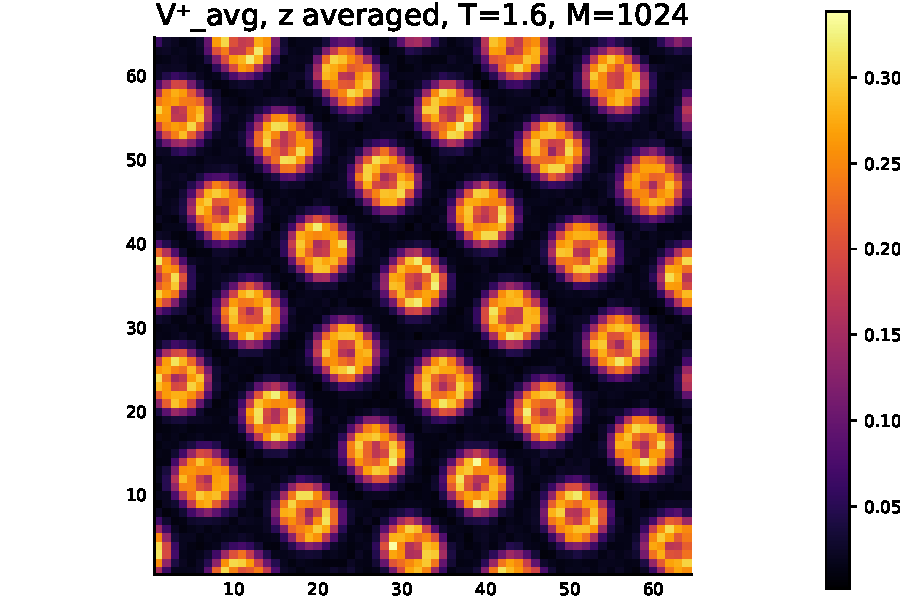
\includegraphics[width=\textwidth]{hex_lattice_V.pdf}
        \caption{\label{fig:Vor:Symm:SF:hex:V}}
    \end{subfigure}
    \hspace{2em}
    \begin{subfigure}[b]{\fractionwidth\textwidth}
        \centering
        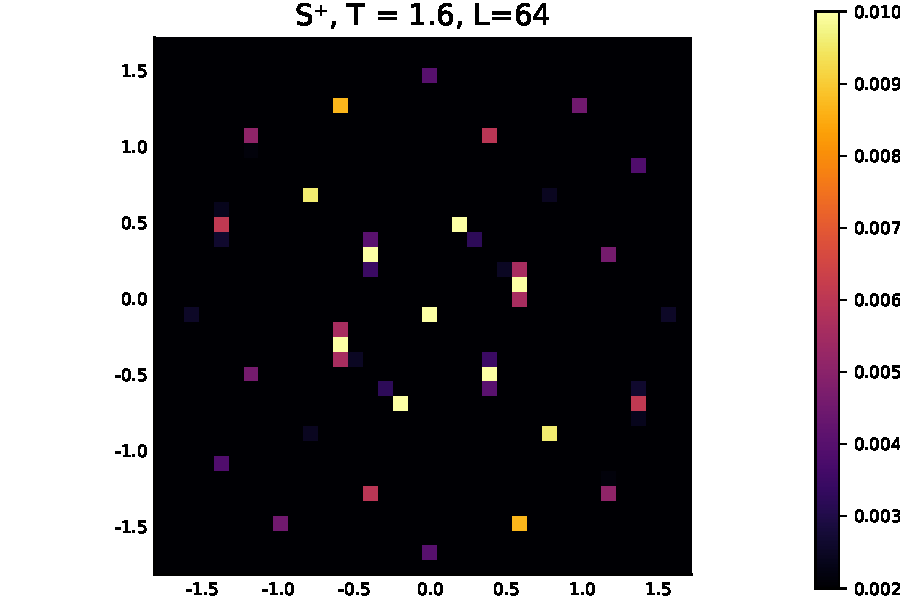
\includegraphics[width=\textwidth]{hex_lattice_S.pdf}
        \caption{\label{fig:Vor:Symm:SF:hex:S}}
    \end{subfigure}
    \caption{Plots of vorticity of the $+$-component of a $p+ip$ superconductor system. Figure~\protect\subref{fig:Vor:Symm:SF:hex:V} shows a plot of the real space vorticity which corresponds to a thermal average of a discretized version of $w(\v{r}_\perp)$ from Eq.~\eqref{eq:Vor:Symm:SF:Cont:unnormalized}. Fig.~\protect\subref{fig:Vor:Symm:SF:hex:S} shows the corresponding structure function which shows a creat hexagonal structure of the vortex line lattice.}
    \label{fig:Vor:Symm:SF:hex}
\end{figure}

\subsection{Angular histogram}

Building on the idea of measuring a specific point in the structure function to signify a structural transition we developed an angular histogram approach that is robust towards rotations of the
vortex lattice. We found this to be important in measuring the transition from a hexagonal to a square vortex lattice since the angular symmetry of the model allowed the hexagonal vortex lattice to
freeze in various directions. To combat this rotation, we built a histogram of the angular distance between peaks in the structure function over several \ac{mc} steps. For a hexagonal
lattice, such a histogram is peaked at the bin containing  the angular distance $\pi/3$, while a square lattice would be peaked at $\pi/2$. Plotting these bins of angular distance over various
temperatures, we were able to measure the transition from the square to the hexagonal lattice as seen in Figure~\ref{fig:Vor:Symm:AH:histPrTemp}.

\begin{figure}[h]
    \centering
    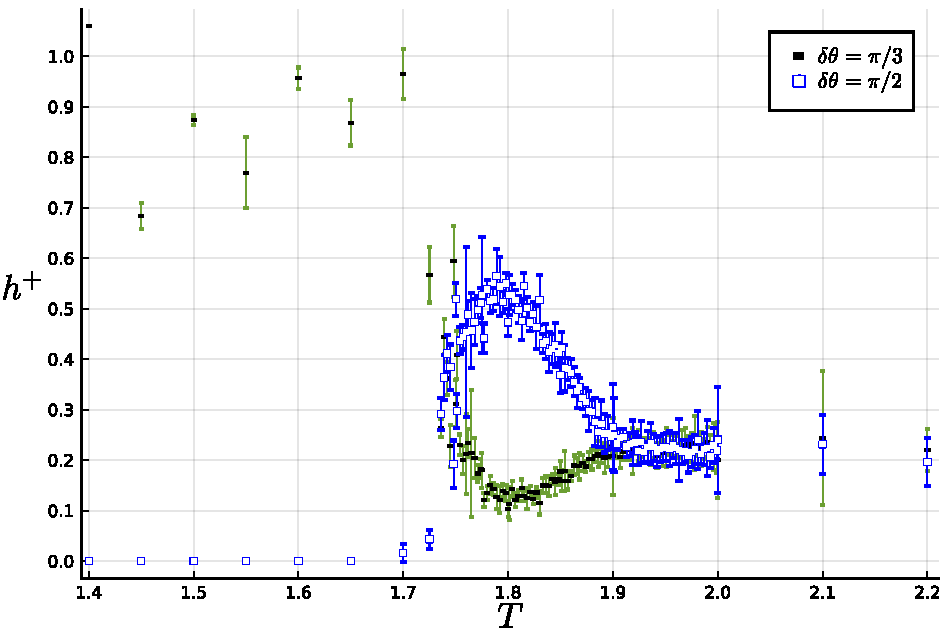
\includegraphics[width=.8\textwidth]{hist_plot.pdf}
    \caption{Plot of the bins of angular distance $\delta\theta = \pi/3$ and $\delta\theta = \pi/2$, as a function of simulation temperature.}
    \label{fig:Vor:Symm:AH:histPrTemp}
\end{figure}

The histogram was constructed algorithmically by creating a set of angular distances between peaks of the structure function for each \ac{mc} step. We first found the radius where the peaks were
located by searching the average structure function over the entire \ac{mc} series, within a specified radius interval for the radius $\rho_m$ that produced the largest value of the
discretization of the integral
\begin{equation}
    \label{eq:Vor:Symm:AH:searchIntegral}
    \int_0^{2\pi}\!\!\!\!\!\!\mathrm{d}\theta\; S(\rho,\theta),
\end{equation}
where $S(\rho,\theta)$ is the structure function given in polar coordinates about the Bragg-point $\v{k}_\perp = \v{0}$. The entire series of \ac{mc} data was then blocked into sections
containing $\Delta\tau$ numbers of individual \ac{mc} measurements of the structure function. Each such interval of structure function measurements were then averaged over to yields separate
averaged measurements of the structure function. This blocking is absolutely necessary in order to reveal the hidden vortex lattice from the noise. From each block $t$,
a structure function ring $S^t(\theta)$ was then created by selecting the highest value of the blocked structure function over a ribbon centered at radius $\rho_m$ such that
\begin{equation}
    \label{eq:Vor:Symm:AH:ribbonMaximum}
    S^t(\theta) = \max_{\rho_m-\delta\rho\leq\rho\leq\rho_m+\delta\rho}\{S^t(\rho,\theta)\}.
\end{equation}

A collection of $n$ peaks $P^t = \{\theta^p\}$ was then found for each block by finding the highest possible $S_m$ such that $S^t(\theta)$ crossed the line $S_m$ $n$ times. From this set of peaks,
then all possible distances between these peak positions were constructed by
\begin{equation}
    \label{eq:Vor:Symm:AH:mutualDistances}
    \Theta^t = \{\delta\theta_{ij} = |\theta^p_i-\theta^p_j|\quad|\quad i\neq j,\;\theta_i^p,\theta_j^p\in P^t\}.
\end{equation}
Let $\Theta = \bigcup_t\Theta^t$ be the union of all block sets of mutual angular peak distances. The final histogram $h$ was then constructed based on all of the distances in $\Theta$. Let the bin
in this histogram of the interval $[0,2\pi)$ that contains the angular distance $\delta\theta$ be denoted $\Delta\delta\theta$ such that 
\begin{equation}
    \label{eq:Vor:Symm:AH:mutualDistancesBin}
    \Delta\delta\theta = [\delta\theta-\delta\theta_-,\delta\theta+\delta\theta_+),
\end{equation}
for some non-negative $\delta\theta_-$ and $\delta\theta_+$. The value of the histogram $h(\Delta\delta\theta)$ at this bin was then calculated by
\begin{equation}
    \label{eq:Vor:Symm:AH:histogramDef}
    h(\Delta\delta\theta) = \frac{1}{\abs{\Delta\delta\theta}\abs{\Theta}}\sum_{\delta\theta'\in\Theta}\delta_{\delta\theta'\in\Delta\delta\theta},
\end{equation}
where $\abs{\Delta\delta\theta}$ is the size of bin $\Delta\delta\theta$, $\abs{\Theta}$ is the number of mutual distances $\delta\theta'$ in $\Theta$
and $\delta_{\delta\theta'\in\Delta\delta\theta}$ is the Kronecker delta function defined as
\begin{equation}
    \label{eq:Vor:Symm:AH:kroneckerDelta}
    \delta_{\delta\theta'\in\Delta\delta\theta} = \left\{
    \begin{array}{lr}
        1 & : \delta\theta'\in\Delta\delta\theta \\
        0 & : \delta\theta'\notin\Delta\delta\theta
    \end{array}\right. .
\end{equation}

An example of the resulting histogram from calculating $h(\Delta\delta\theta)$, given equal size of the $\Delta\delta\theta$ intervals is shown in Figure~\ref{fig:Vor:Symm:AH:histogram}.
In this figure we observe a large peak at $\delta\theta = \pi/2 \approx 1.6$. This correlation comes from the fact that there are $4$ peaks in the structure function
that are equidistant to eachother in angular distance from the origin. From this we draw the conclusion that the histogram represents a signature of a square vortex
lattice. The even larger peak at $\delta\theta = \pi$ comes from a mathematical symmetry of the 2D Fourier transform
that says that $\mathcal{F}(\v{k}) = \mathcal{F}(-\v{k})^\ast$. The small peak at $\delta\theta = 3\pi/2$ is a remnant of the peak at $\pi/2$, while the peak at low $\delta\theta$
is a artiface coming from noise in the data.

\begin{figure}[hb]
    \centering
    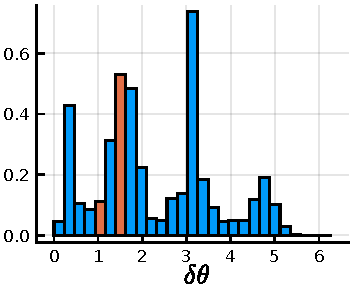
\includegraphics[width=.7\textwidth]{hist_square.pdf}
    \caption{Plot of the bins of $h$ in Eq.~\eqref{eq:Vor:Symm:AH:histogramDef} for a simulation of a square vortex lattice.
    The bins corresponding to $\delta\theta = \pi/3$ and $\delta\theta = \pi/2$ are colored orange to mark the main contributions from
    a triangular- and square lattice respectivly.}
    \label{fig:Vor:Symm:AH:histogram}
\end{figure}

% Structure function
% Peak histogram

